\documentclass[1p]{elsarticle_modified}
%\bibliographystyle{elsarticle-num}

%\usepackage[colorlinks]{hyperref}
%\usepackage{abbrmath_seonhwa} %\Abb, \Ascr, \Acal ,\Abf, \Afrak
\usepackage{amsfonts}
\usepackage{amssymb}
\usepackage{amsmath}
\usepackage{amsthm}
\usepackage{scalefnt}
\usepackage{amsbsy}
\usepackage{kotex}
\usepackage{caption}
\usepackage{subfig}
\usepackage{color}
\usepackage{graphicx}
\usepackage{xcolor} %% white, black, red, green, blue, cyan, magenta, yellow
\usepackage{float}
\usepackage{setspace}
\usepackage{hyperref}

\usepackage{tikz}
\usetikzlibrary{arrows}

\usepackage{multirow}
\usepackage{array} % fixed length table
\usepackage{hhline}

%%%%%%%%%%%%%%%%%%%%%
\makeatletter
\renewcommand*\env@matrix[1][\arraystretch]{%
	\edef\arraystretch{#1}%
	\hskip -\arraycolsep
	\let\@ifnextchar\new@ifnextchar
	\array{*\c@MaxMatrixCols c}}
\makeatother %https://tex.stackexchange.com/questions/14071/how-can-i-increase-the-line-spacing-in-a-matrix
%%%%%%%%%%%%%%%

\usepackage[normalem]{ulem}

\newcommand{\msout}[1]{\ifmmode\text{\sout{\ensuremath{#1}}}\else\sout{#1}\fi}
%SOURCE: \msout is \stkout macro in https://tex.stackexchange.com/questions/20609/strikeout-in-math-mode

\newcommand{\cancel}[1]{
	\ifmmode
	{\color{red}\msout{#1}}
	\else
	{\color{red}\sout{#1}}
	\fi
}

\newcommand{\add}[1]{
	{\color{blue}\uwave{#1}}
}

\newcommand{\replace}[2]{
	\ifmmode
	{\color{red}\msout{#1}}{\color{blue}\uwave{#2}}
	\else
	{\color{red}\sout{#1}}{\color{blue}\uwave{#2}}
	\fi
}

\newcommand{\Sol}{\mathcal{S}} %segment
\newcommand{\D}{D} %diagram
\newcommand{\A}{\mathcal{A}} %arc


%%%%%%%%%%%%%%%%%%%%%%%%%%%%%5 test

\def\sl{\operatorname{\textup{SL}}(2,\Cbb)}
\def\psl{\operatorname{\textup{PSL}}(2,\Cbb)}
\def\quan{\mkern 1mu \triangleright \mkern 1mu}

\theoremstyle{definition}
\newtheorem{thm}{Theorem}[section]
\newtheorem{prop}[thm]{Proposition}
\newtheorem{lem}[thm]{Lemma}
\newtheorem{ques}[thm]{Question}
\newtheorem{cor}[thm]{Corollary}
\newtheorem{defn}[thm]{Definition}
\newtheorem{exam}[thm]{Example}
\newtheorem{rmk}[thm]{Remark}
\newtheorem{alg}[thm]{Algorithm}

\newcommand{\I}{\sqrt{-1}}
\begin{document}

%\begin{frontmatter}
%
%\title{Boundary parabolic representations of knots up to 8 crossings}
%
%%% Group authors per affiliation:
%\author{Yunhi Cho} 
%\address{Department of Mathematics, University of Seoul, Seoul, Korea}
%\ead{yhcho@uos.ac.kr}
%
%
%\author{Seonhwa Kim} %\fnref{s_kim}}
%\address{Center for Geometry and Physics, Institute for Basic Science, Pohang, 37673, Korea}
%\ead{ryeona17@ibs.re.kr}
%
%\author{Hyuk Kim}
%\address{Department of Mathematical Sciences, Seoul National University, Seoul 08826, Korea}
%\ead{hyukkim@snu.ac.kr}
%
%\author{Seokbeom Yoon}
%\address{Department of Mathematical Sciences, Seoul National University, Seoul, 08826,  Korea}
%\ead{sbyoon15@snu.ac.kr}
%
%\begin{abstract}
%We find all boundary parabolic representation of knots up to 8 crossings.
%
%\end{abstract}
%\begin{keyword}
%    \MSC[2010] 57M25 
%\end{keyword}
%
%\end{frontmatter}

%\linenumbers
%\tableofcontents
%
\newcommand\colored[1]{\textcolor{white}{\rule[-0.35ex]{0.8em}{1.4ex}}\kern-0.8em\color{red} #1}%
%\newcommand\colored[1]{\textcolor{white}{ #1}\kern-2.17ex	\textcolor{white}{ #1}\kern-1.81ex	\textcolor{white}{ #1}\kern-2.15ex\color{red}#1	}

{\Large $\underline{12n_{0128}~(K12n_{0128})}$}

\setlength{\tabcolsep}{10pt}
\renewcommand{\arraystretch}{1.6}
\vspace{1cm}\begin{tabular}{m{100pt}>{\centering\arraybackslash}m{274pt}}
\multirow{5}{120pt}{
	\centering
	\includegraphics[width=112pt]{../../../GIT/diagram.site/Diagrams/png/2217_12n_0128.png}\\
\ \ \ A knot diagram\footnotemark}&
\allowdisplaybreaks
\textbf{Linearized knot diagam} \\
\cline{2-2}
 &
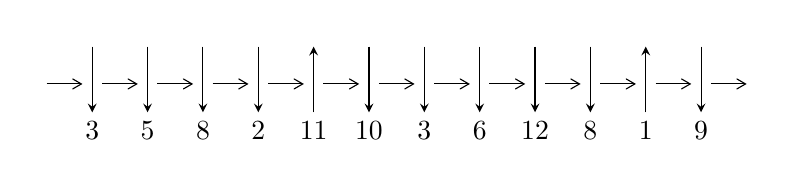
\begin{tikzpicture}[x=20pt, y=17pt]
	% nodes
	\node (C0) at (0, 0) {};
	\node (C1) at (1, 0) {};
	\node (C1U) at (1, +1) {};
	\node (C1D) at (1, -1) {3};

	\node (C2) at (2, 0) {};
	\node (C2U) at (2, +1) {};
	\node (C2D) at (2, -1) {5};

	\node (C3) at (3, 0) {};
	\node (C3U) at (3, +1) {};
	\node (C3D) at (3, -1) {8};

	\node (C4) at (4, 0) {};
	\node (C4U) at (4, +1) {};
	\node (C4D) at (4, -1) {2};

	\node (C5) at (5, 0) {};
	\node (C5U) at (5, +1) {};
	\node (C5D) at (5, -1) {11};

	\node (C6) at (6, 0) {};
	\node (C6U) at (6, +1) {};
	\node (C6D) at (6, -1) {10};

	\node (C7) at (7, 0) {};
	\node (C7U) at (7, +1) {};
	\node (C7D) at (7, -1) {3};

	\node (C8) at (8, 0) {};
	\node (C8U) at (8, +1) {};
	\node (C8D) at (8, -1) {6};

	\node (C9) at (9, 0) {};
	\node (C9U) at (9, +1) {};
	\node (C9D) at (9, -1) {12};

	\node (C10) at (10, 0) {};
	\node (C10U) at (10, +1) {};
	\node (C10D) at (10, -1) {8};

	\node (C11) at (11, 0) {};
	\node (C11U) at (11, +1) {};
	\node (C11D) at (11, -1) {1};

	\node (C12) at (12, 0) {};
	\node (C12U) at (12, +1) {};
	\node (C12D) at (12, -1) {9};
	\node (C13) at (13, 0) {};

	% arrows
	\draw[->,>={angle 60}]
	(C0) edge (C1) (C1) edge (C2) (C2) edge (C3) (C3) edge (C4) (C4) edge (C5) (C5) edge (C6) (C6) edge (C7) (C7) edge (C8) (C8) edge (C9) (C9) edge (C10) (C10) edge (C11) (C11) edge (C12) (C12) edge (C13) ;	\draw[->,>=stealth]
	(C1U) edge (C1D) (C2U) edge (C2D) (C3U) edge (C3D) (C4U) edge (C4D) (C5D) edge (C5U) (C6U) edge (C6D) (C7U) edge (C7D) (C8U) edge (C8D) (C9U) edge (C9D) (C10U) edge (C10D) (C11D) edge (C11U) (C12U) edge (C12D) ;
	\end{tikzpicture} \\
\hhline{~~} \\& 
\textbf{Solving Sequence} \\ \cline{2-2} 
 &
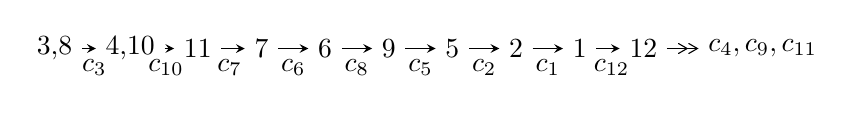
\begin{tikzpicture}[x=23pt, y=7pt]
	% node
	\node (A0) at (-1/8, 0) {3,8};
	\node (A1) at (17/16, 0) {4,10};
	\node (A2) at (17/8, 0) {11};
	\node (A3) at (25/8, 0) {7};
	\node (A4) at (33/8, 0) {6};
	\node (A5) at (41/8, 0) {9};
	\node (A6) at (49/8, 0) {5};
	\node (A7) at (57/8, 0) {2};
	\node (A8) at (65/8, 0) {1};
	\node (A9) at (73/8, 0) {12};
	\node (C1) at (1/2, -1) {$c_{3}$};
	\node (C2) at (13/8, -1) {$c_{10}$};
	\node (C3) at (21/8, -1) {$c_{7}$};
	\node (C4) at (29/8, -1) {$c_{6}$};
	\node (C5) at (37/8, -1) {$c_{8}$};
	\node (C6) at (45/8, -1) {$c_{5}$};
	\node (C7) at (53/8, -1) {$c_{2}$};
	\node (C8) at (61/8, -1) {$c_{1}$};
	\node (C9) at (69/8, -1) {$c_{12}$};
	\node (A10) at (11, 0) {$c_{4},c_{9},c_{11}$};

	% edge
	\draw[->,>=stealth]	
	(A0) edge (A1) (A1) edge (A2) (A2) edge (A3) (A3) edge (A4) (A4) edge (A5) (A5) edge (A6) (A6) edge (A7) (A7) edge (A8) (A8) edge (A9) ;
	\draw[->>,>={angle 60}]	
	(A9) edge (A10);
\end{tikzpicture} \\ 

\end{tabular} \\

\footnotetext{
The image of knot diagram is generated by the software ``\textbf{Draw programme}" developed by Andrew Bartholomew(\url{http://www.layer8.co.uk/maths/draw/index.htm\#Running-draw}), where we modified some parts for our purpose(\url{https://github.com/CATsTAILs/LinksPainter}).
}\phantom \\ \newline 
\centering \textbf{Ideals for irreducible components\footnotemark of $X_{\text{par}}$} 
 
\begin{align*}
I^u_{1}&=\langle 
1.10179\times10^{326} u^{84}+4.59940\times10^{326} u^{83}+\cdots+6.70794\times10^{327} b+9.84549\times10^{328},\\
\phantom{I^u_{1}}&\phantom{= \langle  }-1.92301\times10^{326} u^{84}-4.87952\times10^{326} u^{83}+\cdots+2.68317\times10^{328} a-1.80541\times10^{329},\\
\phantom{I^u_{1}}&\phantom{= \langle  }u^{85}+3 u^{84}+\cdots+2560 u-512\rangle \\
I^u_{2}&=\langle 
b^2-2 b u-3 b+8 u+13,\;a,\;u^2+u-1\rangle \\
\\
I^v_{1}&=\langle 
a,\;-117084 v^8-101146 v^7+\cdots+178147 b-213819,\\
\phantom{I^v_{1}}&\phantom{= \langle  }v^9+v^8+12 v^7+7 v^6+37 v^5- v^4+10 v^2+5 v+1\rangle \\
\end{align*}
\raggedright * 3 irreducible components of $\dim_{\mathbb{C}}=0$, with total 98 representations.\\
\footnotetext{All coefficients of polynomials are rational numbers. But the coefficients are sometimes approximated in decimal forms when there is not enough margin.}
\newpage
\renewcommand{\arraystretch}{1}
\centering \section*{I. $I^u_{1}= \langle 1.10\times10^{326} u^{84}+4.60\times10^{326} u^{83}+\cdots+6.71\times10^{327} b+9.85\times10^{328},\;-1.92\times10^{326} u^{84}-4.88\times10^{326} u^{83}+\cdots+2.68\times10^{328} a-1.81\times10^{329},\;u^{85}+3 u^{84}+\cdots+2560 u-512 \rangle$}
\flushleft \textbf{(i) Arc colorings}\\
\begin{tabular}{m{7pt} m{180pt} m{7pt} m{180pt} }
\flushright $a_{3}=$&$\begin{pmatrix}1\\0\end{pmatrix}$ \\
\flushright $a_{8}=$&$\begin{pmatrix}0\\u\end{pmatrix}$ \\
\flushright $a_{4}=$&$\begin{pmatrix}1\\u^2\end{pmatrix}$ \\
\flushright $a_{10}=$&$\begin{pmatrix}0.00716693 u^{84}+0.0181856 u^{83}+\cdots-41.0816 u+6.72864\\-0.0164251 u^{84}-0.0685666 u^{83}+\cdots+14.1484 u-14.6774\end{pmatrix}$ \\
\flushright $a_{11}=$&$\begin{pmatrix}0.00716693 u^{84}+0.0181856 u^{83}+\cdots-41.0816 u+6.72864\\-0.0173695 u^{84}-0.0700008 u^{83}+\cdots+26.3047 u-16.3747\end{pmatrix}$ \\
\flushright $a_{7}=$&$\begin{pmatrix}u\\u\end{pmatrix}$ \\
\flushright $a_{6}=$&$\begin{pmatrix}0.0128640 u^{84}+0.0390675 u^{83}+\cdots-60.0504 u+9.18109\\0.0370542 u^{84}+0.136353 u^{83}+\cdots-145.401 u+47.2282\end{pmatrix}$ \\
\flushright $a_{9}=$&$\begin{pmatrix}-0.0104888 u^{84}-0.0265281 u^{83}+\cdots+86.9445 u-14.0203\\0.00275780 u^{84}+0.00808818 u^{83}+\cdots+16.3180 u-2.98126\end{pmatrix}$ \\
\flushright $a_{5}=$&$\begin{pmatrix}0.00825383 u^{84}+0.0201646 u^{83}+\cdots-65.1654 u+10.2484\\-0.00335614 u^{84}-0.00827244 u^{83}+\cdots+37.7731 u-6.12557\end{pmatrix}$ \\
\flushright $a_{2}=$&$\begin{pmatrix}0.00825383 u^{84}+0.0201646 u^{83}+\cdots-65.1654 u+10.2484\\0.00223501 u^{84}+0.00636347 u^{83}+\cdots-21.7790 u+3.77196\end{pmatrix}$ \\
\flushright $a_{1}=$&$\begin{pmatrix}0.0104888 u^{84}+0.0265281 u^{83}+\cdots-86.9445 u+14.0203\\0.00223501 u^{84}+0.00636347 u^{83}+\cdots-21.7790 u+3.77196\end{pmatrix}$ \\
\flushright $a_{12}=$&$\begin{pmatrix}-0.000908687 u^{84}-0.00204367 u^{83}+\cdots-16.4201 u+3.85488\\-0.0185413 u^{84}-0.0750717 u^{83}+\cdots-7.29914 u-9.22684\end{pmatrix}$\\&\end{tabular}
\flushleft \textbf{(ii) Obstruction class $= -1$}\\~\\
\flushleft \textbf{(iii) Cusp Shapes $= 0.381801 u^{84}+1.38285 u^{83}+\cdots-1273.67 u+380.918$}\\~\\
\newpage\renewcommand{\arraystretch}{1}
\flushleft \textbf{(iv) u-Polynomials at the component}\newline \\
\begin{tabular}{m{50pt}|m{274pt}}
Crossings & \hspace{64pt}u-Polynomials at each crossing \\
\hline $$\begin{aligned}c_{1}\end{aligned}$$&$\begin{aligned}
&u^{85}+38 u^{84}+\cdots-213 u+1
\end{aligned}$\\
\hline $$\begin{aligned}c_{2},c_{4}\end{aligned}$$&$\begin{aligned}
&u^{85}-12 u^{84}+\cdots- u+1
\end{aligned}$\\
\hline $$\begin{aligned}c_{3},c_{7}\end{aligned}$$&$\begin{aligned}
&u^{85}-3 u^{84}+\cdots+2560 u+512
\end{aligned}$\\
\hline $$\begin{aligned}c_{5}\end{aligned}$$&$\begin{aligned}
&u^{85}+3 u^{84}+\cdots+112806 u+16279
\end{aligned}$\\
\hline $$\begin{aligned}c_{6}\end{aligned}$$&$\begin{aligned}
&u^{85}- u^{84}+\cdots+28266 u+22877
\end{aligned}$\\
\hline $$\begin{aligned}c_{8}\end{aligned}$$&$\begin{aligned}
&u^{85}-4 u^{84}+\cdots-5 u+1
\end{aligned}$\\
\hline $$\begin{aligned}c_{9},c_{12}\end{aligned}$$&$\begin{aligned}
&u^{85}-4 u^{84}+\cdots+7 u+1
\end{aligned}$\\
\hline $$\begin{aligned}c_{10}\end{aligned}$$&$\begin{aligned}
&u^{85}-8 u^{84}+\cdots+192 u+16
\end{aligned}$\\
\hline $$\begin{aligned}c_{11}\end{aligned}$$&$\begin{aligned}
&u^{85}-38 u^{84}+\cdots+27 u+1
\end{aligned}$\\
\hline
\end{tabular}\\~\\
\newpage\renewcommand{\arraystretch}{1}
\flushleft \textbf{(v) Riley Polynomials at the component}\newline \\
\begin{tabular}{m{50pt}|m{274pt}}
Crossings & \hspace{64pt}Riley Polynomials at each crossing \\
\hline $$\begin{aligned}c_{1}\end{aligned}$$&$\begin{aligned}
&y^{85}+30 y^{84}+\cdots+27491 y-1
\end{aligned}$\\
\hline $$\begin{aligned}c_{2},c_{4}\end{aligned}$$&$\begin{aligned}
&y^{85}-38 y^{84}+\cdots-213 y-1
\end{aligned}$\\
\hline $$\begin{aligned}c_{3},c_{7}\end{aligned}$$&$\begin{aligned}
&y^{85}+51 y^{84}+\cdots-3932160 y-262144
\end{aligned}$\\
\hline $$\begin{aligned}c_{5}\end{aligned}$$&$\begin{aligned}
&y^{85}-81 y^{84}+\cdots+5075593862 y-265005841
\end{aligned}$\\
\hline $$\begin{aligned}c_{6}\end{aligned}$$&$\begin{aligned}
&y^{85}-57 y^{84}+\cdots-21266860578 y-523357129
\end{aligned}$\\
\hline $$\begin{aligned}c_{8}\end{aligned}$$&$\begin{aligned}
&y^{85}-22 y^{84}+\cdots+31 y-1
\end{aligned}$\\
\hline $$\begin{aligned}c_{9},c_{12}\end{aligned}$$&$\begin{aligned}
&y^{85}+38 y^{84}+\cdots+27 y-1
\end{aligned}$\\
\hline $$\begin{aligned}c_{10}\end{aligned}$$&$\begin{aligned}
&y^{85}+20 y^{84}+\cdots+12160 y-256
\end{aligned}$\\
\hline $$\begin{aligned}c_{11}\end{aligned}$$&$\begin{aligned}
&y^{85}+22 y^{84}+\cdots+1735 y-1
\end{aligned}$\\
\hline
\end{tabular}\\~\\
\newpage\flushleft \textbf{(vi) Complex Volumes and Cusp Shapes}
$$\begin{array}{c|c|c}  
\text{Solutions to }I^u_{1}& \I (\text{vol} + \sqrt{-1}CS) & \text{Cusp shape}\\
 \hline 
\begin{aligned}
u &= \phantom{-}1.079250 + 0.084385 I \\
a &= \phantom{-}0.314607 - 0.642851 I \\
b &= -0.263280 + 0.005137 I\end{aligned}
 & -1.013250 + 0.170939 I & \phantom{-0.000000 } 0 \\ \hline\begin{aligned}
u &= \phantom{-}1.079250 - 0.084385 I \\
a &= \phantom{-}0.314607 + 0.642851 I \\
b &= -0.263280 - 0.005137 I\end{aligned}
 & -1.013250 - 0.170939 I & \phantom{-0.000000 } 0 \\ \hline\begin{aligned}
u &= -1.111280 + 0.071551 I \\
a &= \phantom{-}0.643580 - 0.926472 I \\
b &= \phantom{-}0.321561 - 0.222730 I\end{aligned}
 & \phantom{-}3.33969 + 2.83227 I & \phantom{-0.000000 } 0 \\ \hline\begin{aligned}
u &= -1.111280 - 0.071551 I \\
a &= \phantom{-}0.643580 + 0.926472 I \\
b &= \phantom{-}0.321561 + 0.222730 I\end{aligned}
 & \phantom{-}3.33969 - 2.83227 I & \phantom{-0.000000 } 0 \\ \hline\begin{aligned}
u &= -0.129045 + 1.113980 I \\
a &= \phantom{-}1.74054 - 0.17640 I \\
b &= \phantom{-}1.96919 - 0.18618 I\end{aligned}
 & \phantom{-}0.094102 - 1.056740 I & \phantom{-0.000000 } 0 \\ \hline\begin{aligned}
u &= -0.129045 - 1.113980 I \\
a &= \phantom{-}1.74054 + 0.17640 I \\
b &= \phantom{-}1.96919 + 0.18618 I\end{aligned}
 & \phantom{-}0.094102 + 1.056740 I & \phantom{-0.000000 } 0 \\ \hline\begin{aligned}
u &= -0.210154 + 1.114290 I \\
a &= -0.839901 - 0.413606 I \\
b &= -1.63994 - 1.01283 I\end{aligned}
 & -3.15620 + 2.51605 I & \phantom{-0.000000 } 0 \\ \hline\begin{aligned}
u &= -0.210154 - 1.114290 I \\
a &= -0.839901 + 0.413606 I \\
b &= -1.63994 + 1.01283 I\end{aligned}
 & -3.15620 - 2.51605 I & \phantom{-0.000000 } 0 \\ \hline\begin{aligned}
u &= \phantom{-}0.433540 + 1.050740 I \\
a &= \phantom{-}0.587198 + 0.587186 I \\
b &= \phantom{-}0.993744 + 0.855462 I\end{aligned}
 & \phantom{-}0.982642 + 0.642938 I & \phantom{-0.000000 } 0 \\ \hline\begin{aligned}
u &= \phantom{-}0.433540 - 1.050740 I \\
a &= \phantom{-}0.587198 - 0.587186 I \\
b &= \phantom{-}0.993744 - 0.855462 I\end{aligned}
 & \phantom{-}0.982642 - 0.642938 I & \phantom{-0.000000 } 0\\
 \hline 
 \end{array}$$\newpage$$\begin{array}{c|c|c}  
\text{Solutions to }I^u_{1}& \I (\text{vol} + \sqrt{-1}CS) & \text{Cusp shape}\\
 \hline 
\begin{aligned}
u &= -0.257695 + 1.109990 I \\
a &= -0.04586 - 1.76277 I \\
b &= \phantom{-}0.070299 - 0.881993 I\end{aligned}
 & -1.09681 + 2.37421 I & \phantom{-0.000000 } 0 \\ \hline\begin{aligned}
u &= -0.257695 - 1.109990 I \\
a &= -0.04586 + 1.76277 I \\
b &= \phantom{-}0.070299 + 0.881993 I\end{aligned}
 & -1.09681 - 2.37421 I & \phantom{-0.000000 } 0 \\ \hline\begin{aligned}
u &= \phantom{-}0.262541 + 1.168940 I \\
a &= -0.497533 + 0.412605 I \\
b &= -1.021630 - 0.852821 I\end{aligned}
 & \phantom{-}2.10819 - 3.90878 I & \phantom{-0.000000 } 0 \\ \hline\begin{aligned}
u &= \phantom{-}0.262541 - 1.168940 I \\
a &= -0.497533 - 0.412605 I \\
b &= -1.021630 + 0.852821 I\end{aligned}
 & \phantom{-}2.10819 + 3.90878 I & \phantom{-0.000000 } 0 \\ \hline\begin{aligned}
u &= \phantom{-}0.218930 + 1.186920 I \\
a &= \phantom{-}0.438793 + 0.422340 I \\
b &= \phantom{-}1.29909 - 1.31313 I\end{aligned}
 & \phantom{-}2.18193 - 1.17088 I & \phantom{-0.000000 } 0 \\ \hline\begin{aligned}
u &= \phantom{-}0.218930 - 1.186920 I \\
a &= \phantom{-}0.438793 - 0.422340 I \\
b &= \phantom{-}1.29909 + 1.31313 I\end{aligned}
 & \phantom{-}2.18193 + 1.17088 I & \phantom{-0.000000 } 0 \\ \hline\begin{aligned}
u &= -0.758522 + 0.188313 I \\
a &= \phantom{-}1.47819 - 0.47702 I \\
b &= \phantom{-}2.18056 + 0.45533 I\end{aligned}
 & -1.13123 - 4.17645 I & -11.8176 + 9.1818 I \\ \hline\begin{aligned}
u &= -0.758522 - 0.188313 I \\
a &= \phantom{-}1.47819 + 0.47702 I \\
b &= \phantom{-}2.18056 - 0.45533 I\end{aligned}
 & -1.13123 + 4.17645 I & -11.8176 - 9.1818 I \\ \hline\begin{aligned}
u &= -0.341078 + 1.170670 I \\
a &= -1.71012 - 0.11107 I \\
b &= -2.09658 - 0.30512 I\end{aligned}
 & -0.41725 + 6.01567 I & \phantom{-0.000000 } 0 \\ \hline\begin{aligned}
u &= -0.341078 - 1.170670 I \\
a &= -1.71012 + 0.11107 I \\
b &= -2.09658 + 0.30512 I\end{aligned}
 & -0.41725 - 6.01567 I & \phantom{-0.000000 } 0\\
 \hline 
 \end{array}$$\newpage$$\begin{array}{c|c|c}  
\text{Solutions to }I^u_{1}& \I (\text{vol} + \sqrt{-1}CS) & \text{Cusp shape}\\
 \hline 
\begin{aligned}
u &= \phantom{-}0.041071 + 1.235810 I \\
a &= \phantom{-}0.35122 + 1.48542 I \\
b &= \phantom{-}0.799108 + 0.646539 I\end{aligned}
 & \phantom{-}3.32593 - 3.12666 I & \phantom{-0.000000 } 0 \\ \hline\begin{aligned}
u &= \phantom{-}0.041071 - 1.235810 I \\
a &= \phantom{-}0.35122 - 1.48542 I \\
b &= \phantom{-}0.799108 - 0.646539 I\end{aligned}
 & \phantom{-}3.32593 + 3.12666 I & \phantom{-0.000000 } 0 \\ \hline\begin{aligned}
u &= -1.206060 + 0.339502 I \\
a &= -0.333951 - 0.966861 I \\
b &= \phantom{-}0.172479 - 0.075194 I\end{aligned}
 & -1.81678 - 5.27916 I & \phantom{-0.000000 } 0 \\ \hline\begin{aligned}
u &= -1.206060 - 0.339502 I \\
a &= -0.333951 + 0.966861 I \\
b &= \phantom{-}0.172479 + 0.075194 I\end{aligned}
 & -1.81678 + 5.27916 I & \phantom{-0.000000 } 0 \\ \hline\begin{aligned}
u &= -0.573407 + 0.367957 I \\
a &= \phantom{-}0.02490 - 1.59180 I \\
b &= \phantom{-}0.90204 - 1.21732 I\end{aligned}
 & -3.03530 - 2.32112 I & -18.2811 + 2.9821 I \\ \hline\begin{aligned}
u &= -0.573407 - 0.367957 I \\
a &= \phantom{-}0.02490 + 1.59180 I \\
b &= \phantom{-}0.90204 + 1.21732 I\end{aligned}
 & -3.03530 + 2.32112 I & -18.2811 - 2.9821 I \\ \hline\begin{aligned}
u &= \phantom{-}0.091692 + 1.317030 I \\
a &= \phantom{-}0.134568 - 0.539810 I \\
b &= \phantom{-}0.21801 + 1.72217 I\end{aligned}
 & \phantom{-}3.52281 - 0.13174 I & \phantom{-0.000000 } 0 \\ \hline\begin{aligned}
u &= \phantom{-}0.091692 - 1.317030 I \\
a &= \phantom{-}0.134568 + 0.539810 I \\
b &= \phantom{-}0.21801 - 1.72217 I\end{aligned}
 & \phantom{-}3.52281 + 0.13174 I & \phantom{-0.000000 } 0 \\ \hline\begin{aligned}
u &= -0.413209 + 1.277050 I \\
a &= -0.33458 + 1.53181 I \\
b &= -0.762037 + 0.868186 I\end{aligned}
 & \phantom{-}2.39077 + 8.65291 I & \phantom{-0.000000 } 0 \\ \hline\begin{aligned}
u &= -0.413209 - 1.277050 I \\
a &= -0.33458 - 1.53181 I \\
b &= -0.762037 - 0.868186 I\end{aligned}
 & \phantom{-}2.39077 - 8.65291 I & \phantom{-0.000000 } 0\\
 \hline 
 \end{array}$$\newpage$$\begin{array}{c|c|c}  
\text{Solutions to }I^u_{1}& \I (\text{vol} + \sqrt{-1}CS) & \text{Cusp shape}\\
 \hline 
\begin{aligned}
u &= \phantom{-}0.312068 + 1.307370 I \\
a &= -0.183364 - 0.488108 I \\
b &= -0.82725 + 1.90837 I\end{aligned}
 & \phantom{-}3.08119 - 5.55867 I & \phantom{-0.000000 } 0 \\ \hline\begin{aligned}
u &= \phantom{-}0.312068 - 1.307370 I \\
a &= -0.183364 + 0.488108 I \\
b &= -0.82725 - 1.90837 I\end{aligned}
 & \phantom{-}3.08119 + 5.55867 I & \phantom{-0.000000 } 0 \\ \hline\begin{aligned}
u &= -0.459021 + 0.459779 I \\
a &= -1.51990 - 0.28470 I \\
b &= -2.42465 - 1.18474 I\end{aligned}
 & -3.21369 + 0.63442 I & -17.2881 - 6.4476 I \\ \hline\begin{aligned}
u &= -0.459021 - 0.459779 I \\
a &= -1.51990 + 0.28470 I \\
b &= -2.42465 + 1.18474 I\end{aligned}
 & -3.21369 - 0.63442 I & -17.2881 + 6.4476 I \\ \hline\begin{aligned}
u &= \phantom{-}0.634951 + 0.073211 I \\
a &= \phantom{-}0.544294 - 0.378389 I \\
b &= -0.448469 + 0.000623 I\end{aligned}
 & -0.938890 - 0.000686 I & -9.17733 + 0.04419 I \\ \hline\begin{aligned}
u &= \phantom{-}0.634951 - 0.073211 I \\
a &= \phantom{-}0.544294 + 0.378389 I \\
b &= -0.448469 - 0.000623 I\end{aligned}
 & -0.938890 + 0.000686 I & -9.17733 - 0.04419 I \\ \hline\begin{aligned}
u &= \phantom{-}1.237320 + 0.581154 I \\
a &= -0.335451 - 0.582811 I \\
b &= -0.266329 - 0.154538 I\end{aligned}
 & \phantom{-}1.88882 + 2.34511 I & \phantom{-0.000000 } 0 \\ \hline\begin{aligned}
u &= \phantom{-}1.237320 - 0.581154 I \\
a &= -0.335451 + 0.582811 I \\
b &= -0.266329 + 0.154538 I\end{aligned}
 & \phantom{-}1.88882 - 2.34511 I & \phantom{-0.000000 } 0 \\ \hline\begin{aligned}
u &= -0.326856 + 1.339410 I \\
a &= \phantom{-}0.750171 - 0.025748 I \\
b &= \phantom{-}1.332330 - 0.310227 I\end{aligned}
 & \phantom{-}4.34006 - 0.60753 I & \phantom{-0.000000 } 0 \\ \hline\begin{aligned}
u &= -0.326856 - 1.339410 I \\
a &= \phantom{-}0.750171 + 0.025748 I \\
b &= \phantom{-}1.332330 + 0.310227 I\end{aligned}
 & \phantom{-}4.34006 + 0.60753 I & \phantom{-0.000000 } 0\\
 \hline 
 \end{array}$$\newpage$$\begin{array}{c|c|c}  
\text{Solutions to }I^u_{1}& \I (\text{vol} + \sqrt{-1}CS) & \text{Cusp shape}\\
 \hline 
\begin{aligned}
u &= -0.143186 + 1.381320 I \\
a &= \phantom{-}0.727087 + 0.371136 I \\
b &= \phantom{-}1.59812 + 0.81572 I\end{aligned}
 & -1.24862 + 7.38729 I & \phantom{-0.000000 } 0 \\ \hline\begin{aligned}
u &= -0.143186 - 1.381320 I \\
a &= \phantom{-}0.727087 - 0.371136 I \\
b &= \phantom{-}1.59812 - 0.81572 I\end{aligned}
 & -1.24862 - 7.38729 I & \phantom{-0.000000 } 0 \\ \hline\begin{aligned}
u &= \phantom{-}0.607638 + 0.026477 I \\
a &= \phantom{-}0.314965 - 0.062706 I \\
b &= \phantom{-}5.61070 + 1.95263 I\end{aligned}
 & -1.01649 + 2.08350 I & -108.2002 - 27.5787 I \\ \hline\begin{aligned}
u &= \phantom{-}0.607638 - 0.026477 I \\
a &= \phantom{-}0.314965 + 0.062706 I \\
b &= \phantom{-}5.61070 - 1.95263 I\end{aligned}
 & -1.01649 - 2.08350 I & -108.2002 + 27.5787 I \\ \hline\begin{aligned}
u &= \phantom{-}0.573976 + 0.144239 I \\
a &= -0.630973 + 0.039451 I \\
b &= -3.74818 - 1.33751 I\end{aligned}
 & -1.01583 - 1.80194 I & -34.3945 + 9.4437 I \\ \hline\begin{aligned}
u &= \phantom{-}0.573976 - 0.144239 I \\
a &= -0.630973 - 0.039451 I \\
b &= -3.74818 + 1.33751 I\end{aligned}
 & -1.01583 + 1.80194 I & -34.3945 - 9.4437 I \\ \hline\begin{aligned}
u &= \phantom{-}0.581059\phantom{ +0.000000I} \\
a &= \phantom{-}0.632960\phantom{ +0.000000I} \\
b &= -0.432804\phantom{ +0.000000I}\end{aligned}
 & -0.943887\phantom{ +0.000000I} & -9.70520\phantom{ +0.000000I} \\ \hline\begin{aligned}
u &= \phantom{-}0.64849 + 1.26742 I \\
a &= -0.718497 + 0.104136 I \\
b &= -1.213270 + 0.001074 I\end{aligned}
 & \phantom{-}2.43921 - 5.21595 I & \phantom{-0.000000 } 0 \\ \hline\begin{aligned}
u &= \phantom{-}0.64849 - 1.26742 I \\
a &= -0.718497 - 0.104136 I \\
b &= -1.213270 - 0.001074 I\end{aligned}
 & \phantom{-}2.43921 + 5.21595 I & \phantom{-0.000000 } 0 \\ \hline\begin{aligned}
u &= -1.40213 + 0.33857 I \\
a &= \phantom{-}0.330302 + 0.857940 I \\
b &= -0.097754 - 0.133086 I\end{aligned}
 & \phantom{-}0.33638 - 10.54090 I & \phantom{-0.000000 } 0\\
 \hline 
 \end{array}$$\newpage$$\begin{array}{c|c|c}  
\text{Solutions to }I^u_{1}& \I (\text{vol} + \sqrt{-1}CS) & \text{Cusp shape}\\
 \hline 
\begin{aligned}
u &= -1.40213 - 0.33857 I \\
a &= \phantom{-}0.330302 - 0.857940 I \\
b &= -0.097754 + 0.133086 I\end{aligned}
 & \phantom{-}0.33638 + 10.54090 I & \phantom{-0.000000 } 0 \\ \hline\begin{aligned}
u &= -0.056938 + 0.544127 I \\
a &= \phantom{-}0.47075 - 2.43754 I \\
b &= \phantom{-}0.0150861 - 0.0630346 I\end{aligned}
 & -5.59621 - 1.18326 I & -2.58478 - 2.54783 I \\ \hline\begin{aligned}
u &= -0.056938 - 0.544127 I \\
a &= \phantom{-}0.47075 + 2.43754 I \\
b &= \phantom{-}0.0150861 + 0.0630346 I\end{aligned}
 & -5.59621 + 1.18326 I & -2.58478 + 2.54783 I \\ \hline\begin{aligned}
u &= -0.188367 + 0.482280 I \\
a &= \phantom{-}0.01185 + 1.83477 I \\
b &= \phantom{-}0.515477 - 0.218779 I\end{aligned}
 & \phantom{-}1.59907 - 2.42394 I & -1.69948 + 4.54557 I \\ \hline\begin{aligned}
u &= -0.188367 - 0.482280 I \\
a &= \phantom{-}0.01185 - 1.83477 I \\
b &= \phantom{-}0.515477 + 0.218779 I\end{aligned}
 & \phantom{-}1.59907 + 2.42394 I & -1.69948 - 4.54557 I \\ \hline\begin{aligned}
u &= \phantom{-}0.014000 + 0.513349 I \\
a &= -0.98858 + 2.43038 I \\
b &= -0.0540751 + 0.0186456 I\end{aligned}
 & -4.86894 - 7.11123 I & \phantom{-}0.90699 + 6.44296 I \\ \hline\begin{aligned}
u &= \phantom{-}0.014000 - 0.513349 I \\
a &= -0.98858 - 2.43038 I \\
b &= -0.0540751 - 0.0186456 I\end{aligned}
 & -4.86894 + 7.11123 I & \phantom{-}0.90699 - 6.44296 I \\ \hline\begin{aligned}
u &= \phantom{-}1.49443 + 0.02360 I \\
a &= -0.263064 - 0.608348 I \\
b &= \phantom{-}0.056186 + 0.172181 I\end{aligned}
 & \phantom{-}0.90720 - 4.33616 I & \phantom{-0.000000 } 0 \\ \hline\begin{aligned}
u &= \phantom{-}1.49443 - 0.02360 I \\
a &= -0.263064 + 0.608348 I \\
b &= \phantom{-}0.056186 - 0.172181 I\end{aligned}
 & \phantom{-}0.90720 + 4.33616 I & \phantom{-0.000000 } 0 \\ \hline\begin{aligned}
u &= \phantom{-}0.47007 + 1.42149 I \\
a &= \phantom{-}1.025930 - 0.210323 I \\
b &= \phantom{-}1.94222 - 0.59005 I\end{aligned}
 & \phantom{-}3.61530 - 5.88108 I & \phantom{-0.000000 } 0\\
 \hline 
 \end{array}$$\newpage$$\begin{array}{c|c|c}  
\text{Solutions to }I^u_{1}& \I (\text{vol} + \sqrt{-1}CS) & \text{Cusp shape}\\
 \hline 
\begin{aligned}
u &= \phantom{-}0.47007 - 1.42149 I \\
a &= \phantom{-}1.025930 + 0.210323 I \\
b &= \phantom{-}1.94222 + 0.59005 I\end{aligned}
 & \phantom{-}3.61530 + 5.88108 I & \phantom{-0.000000 } 0 \\ \hline\begin{aligned}
u &= -0.129721 + 0.460651 I \\
a &= -0.94046 + 1.36587 I \\
b &= -2.80445 + 1.09956 I\end{aligned}
 & -2.08258 + 2.71217 I & -0.93392 - 9.03807 I \\ \hline\begin{aligned}
u &= -0.129721 - 0.460651 I \\
a &= -0.94046 - 1.36587 I \\
b &= -2.80445 - 1.09956 I\end{aligned}
 & -2.08258 - 2.71217 I & -0.93392 + 9.03807 I \\ \hline\begin{aligned}
u &= -0.69533 + 1.35551 I \\
a &= -1.115150 - 0.202740 I \\
b &= -2.11433 - 0.55269 I\end{aligned}
 & \phantom{-}1.45650 + 12.12210 I & \phantom{-0.000000 } 0 \\ \hline\begin{aligned}
u &= -0.69533 - 1.35551 I \\
a &= -1.115150 + 0.202740 I \\
b &= -2.11433 + 0.55269 I\end{aligned}
 & \phantom{-}1.45650 - 12.12210 I & \phantom{-0.000000 } 0 \\ \hline\begin{aligned}
u &= \phantom{-}0.20084 + 1.51437 I \\
a &= -1.083660 + 0.427485 I \\
b &= -1.88224 + 0.54463 I\end{aligned}
 & \phantom{-}9.43138 - 2.34122 I & \phantom{-0.000000 } 0 \\ \hline\begin{aligned}
u &= \phantom{-}0.20084 - 1.51437 I \\
a &= -1.083660 - 0.427485 I \\
b &= -1.88224 - 0.54463 I\end{aligned}
 & \phantom{-}9.43138 + 2.34122 I & \phantom{-0.000000 } 0 \\ \hline\begin{aligned}
u &= -0.51519 + 1.44160 I \\
a &= \phantom{-}1.189150 + 0.430508 I \\
b &= \phantom{-}2.06507 + 0.51343 I\end{aligned}
 & \phantom{-}8.12807 + 8.74738 I & \phantom{-0.000000 } 0 \\ \hline\begin{aligned}
u &= -0.51519 - 1.44160 I \\
a &= \phantom{-}1.189150 - 0.430508 I \\
b &= \phantom{-}2.06507 - 0.51343 I\end{aligned}
 & \phantom{-}8.12807 - 8.74738 I & \phantom{-0.000000 } 0 \\ \hline\begin{aligned}
u &= -0.67286 + 1.43031 I \\
a &= -0.721546 + 0.163020 I \\
b &= -1.261450 + 0.117391 I\end{aligned}
 & \phantom{-}7.12915 + 3.60494 I & \phantom{-0.000000 } 0\\
 \hline 
 \end{array}$$\newpage$$\begin{array}{c|c|c}  
\text{Solutions to }I^u_{1}& \I (\text{vol} + \sqrt{-1}CS) & \text{Cusp shape}\\
 \hline 
\begin{aligned}
u &= -0.67286 - 1.43031 I \\
a &= -0.721546 - 0.163020 I \\
b &= -1.261450 - 0.117391 I\end{aligned}
 & \phantom{-}7.12915 - 3.60494 I & \phantom{-0.000000 } 0 \\ \hline\begin{aligned}
u &= \phantom{-}0.83986 + 1.36381 I \\
a &= \phantom{-}0.709212 - 0.012362 I \\
b &= \phantom{-}1.255120 - 0.185897 I\end{aligned}
 & \phantom{-}4.36978 - 10.04380 I & \phantom{-0.000000 } 0 \\ \hline\begin{aligned}
u &= \phantom{-}0.83986 - 1.36381 I \\
a &= \phantom{-}0.709212 + 0.012362 I \\
b &= \phantom{-}1.255120 + 0.185897 I\end{aligned}
 & \phantom{-}4.36978 + 10.04380 I & \phantom{-0.000000 } 0 \\ \hline\begin{aligned}
u &= -0.76822 + 1.41143 I \\
a &= \phantom{-}1.028460 + 0.202507 I \\
b &= \phantom{-}2.16194 + 0.54337 I\end{aligned}
 & \phantom{-}3.7759 + 18.1504 I & \phantom{-0.000000 } 0 \\ \hline\begin{aligned}
u &= -0.76822 - 1.41143 I \\
a &= \phantom{-}1.028460 - 0.202507 I \\
b &= \phantom{-}2.16194 - 0.54337 I\end{aligned}
 & \phantom{-}3.7759 - 18.1504 I & \phantom{-0.000000 } 0 \\ \hline\begin{aligned}
u &= \phantom{-}0.56721 + 1.54481 I \\
a &= -0.932269 + 0.216487 I \\
b &= -1.99467 + 0.56349 I\end{aligned}
 & \phantom{-}6.15588 - 11.53790 I & \phantom{-0.000000 } 0 \\ \hline\begin{aligned}
u &= \phantom{-}0.56721 - 1.54481 I \\
a &= -0.932269 - 0.216487 I \\
b &= -1.99467 - 0.56349 I\end{aligned}
 & \phantom{-}6.15588 + 11.53790 I & \phantom{-0.000000 } 0 \\ \hline\begin{aligned}
u &= -1.64677 + 0.04569 I \\
a &= -0.075386 - 0.147225 I \\
b &= \phantom{-}0.0593377 + 0.1023010 I\end{aligned}
 & -8.84126 + 1.96210 I & \phantom{-0.000000 } 0 \\ \hline\begin{aligned}
u &= -1.64677 - 0.04569 I \\
a &= -0.075386 + 0.147225 I \\
b &= \phantom{-}0.0593377 - 0.1023010 I\end{aligned}
 & -8.84126 - 1.96210 I & \phantom{-0.000000 } 0 \\ \hline\begin{aligned}
u &= \phantom{-}0.49039 + 1.61919 I \\
a &= \phantom{-}0.600613 - 0.046493 I \\
b &= \phantom{-}1.53138 - 0.09575 I\end{aligned}
 & \phantom{-}6.55517 - 3.11546 I & \phantom{-0.000000 } 0\\
 \hline 
 \end{array}$$\newpage$$\begin{array}{c|c|c}  
\text{Solutions to }I^u_{1}& \I (\text{vol} + \sqrt{-1}CS) & \text{Cusp shape}\\
 \hline 
\begin{aligned}
u &= \phantom{-}0.49039 - 1.61919 I \\
a &= \phantom{-}0.600613 + 0.046493 I \\
b &= \phantom{-}1.53138 + 0.09575 I\end{aligned}
 & \phantom{-}6.55517 + 3.11546 I & \phantom{-0.000000 } 0 \\ \hline\begin{aligned}
u &= \phantom{-}0.225615 + 0.193490 I \\
a &= \phantom{-}1.41404 + 1.72695 I \\
b &= \phantom{-}0.573669 - 1.131970 I\end{aligned}
 & -0.60683 - 2.35987 I & -1.70647 + 4.72969 I \\ \hline\begin{aligned}
u &= \phantom{-}0.225615 - 0.193490 I \\
a &= \phantom{-}1.41404 - 1.72695 I \\
b &= \phantom{-}0.573669 + 1.131970 I\end{aligned}
 & -0.60683 + 2.35987 I & -1.70647 - 4.72969 I \\ \hline\begin{aligned}
u &= -0.22938 + 1.72989 I \\
a &= -0.626650 + 0.057918 I \\
b &= -1.50572 + 0.17267 I\end{aligned}
 & \phantom{-}7.76106 - 3.97762 I & \phantom{-0.000000 } 0 \\ \hline\begin{aligned}
u &= -0.22938 - 1.72989 I \\
a &= -0.626650 - 0.057918 I \\
b &= -1.50572 - 0.17267 I\end{aligned}
 & \phantom{-}7.76106 + 3.97762 I & \phantom{-0.000000 } 0\\
 \hline 
 \end{array}$$\newpage\newpage\renewcommand{\arraystretch}{1}
\centering \section*{II. $I^u_{2}= \langle b^2-2 b u-3 b+8 u+13,\;a,\;u^2+u-1 \rangle$}
\flushleft \textbf{(i) Arc colorings}\\
\begin{tabular}{m{7pt} m{180pt} m{7pt} m{180pt} }
\flushright $a_{3}=$&$\begin{pmatrix}1\\0\end{pmatrix}$ \\
\flushright $a_{8}=$&$\begin{pmatrix}0\\u\end{pmatrix}$ \\
\flushright $a_{4}=$&$\begin{pmatrix}1\\- u+1\end{pmatrix}$ \\
\flushright $a_{10}=$&$\begin{pmatrix}0\\b\end{pmatrix}$ \\
\flushright $a_{11}=$&$\begin{pmatrix}0\\b\end{pmatrix}$ \\
\flushright $a_{7}=$&$\begin{pmatrix}u\\u\end{pmatrix}$ \\
\flushright $a_{6}=$&$\begin{pmatrix}u\\- b u-2 b+6 u+8\end{pmatrix}$ \\
\flushright $a_{9}=$&$\begin{pmatrix}-2 u+1\\b-3 u-2\end{pmatrix}$ \\
\flushright $a_{5}=$&$\begin{pmatrix}u\\u\end{pmatrix}$ \\
\flushright $a_{2}=$&$\begin{pmatrix}u\\u-1\end{pmatrix}$ \\
\flushright $a_{1}=$&$\begin{pmatrix}2 u-1\\u-1\end{pmatrix}$ \\
\flushright $a_{12}=$&$\begin{pmatrix}-8 b u+5 b\\-5 b u+4 b\end{pmatrix}$\\&\end{tabular}
\flushleft \textbf{(ii) Obstruction class $= 1$}\\~\\
\flushleft \textbf{(iii) Cusp Shapes $= -92 b u+67 b-21 u-44$}\\~\\
\newpage\renewcommand{\arraystretch}{1}
\flushleft \textbf{(iv) u-Polynomials at the component}\newline \\
\begin{tabular}{m{50pt}|m{274pt}}
Crossings & \hspace{64pt}u-Polynomials at each crossing \\
\hline $$\begin{aligned}c_{1}\end{aligned}$$&$\begin{aligned}
&(u^2-3 u+1)^2
\end{aligned}$\\
\hline $$\begin{aligned}c_{2},c_{3}\end{aligned}$$&$\begin{aligned}
&(u^2+u-1)^2
\end{aligned}$\\
\hline $$\begin{aligned}c_{4},c_{7}\end{aligned}$$&$\begin{aligned}
&(u^2- u-1)^2
\end{aligned}$\\
\hline $$\begin{aligned}c_{5},c_{6}\end{aligned}$$&$\begin{aligned}
&u^4-3 u^3+8 u^2-3 u+1
\end{aligned}$\\
\hline $$\begin{aligned}c_{8}\end{aligned}$$&$\begin{aligned}
&(u^2+3 u+1)^2
\end{aligned}$\\
\hline $$\begin{aligned}c_{9}\end{aligned}$$&$\begin{aligned}
&(u^2- u+1)^2
\end{aligned}$\\
\hline $$\begin{aligned}c_{10}\end{aligned}$$&$\begin{aligned}
&u^4
\end{aligned}$\\
\hline $$\begin{aligned}c_{11},c_{12}\end{aligned}$$&$\begin{aligned}
&(u^2+u+1)^2
\end{aligned}$\\
\hline
\end{tabular}\\~\\
\newpage\renewcommand{\arraystretch}{1}
\flushleft \textbf{(v) Riley Polynomials at the component}\newline \\
\begin{tabular}{m{50pt}|m{274pt}}
Crossings & \hspace{64pt}Riley Polynomials at each crossing \\
\hline $$\begin{aligned}c_{1},c_{8}\end{aligned}$$&$\begin{aligned}
&(y^2-7 y+1)^2
\end{aligned}$\\
\hline $$\begin{aligned}c_{2},c_{3},c_{4}\\c_{7}\end{aligned}$$&$\begin{aligned}
&(y^2-3 y+1)^2
\end{aligned}$\\
\hline $$\begin{aligned}c_{5},c_{6}\end{aligned}$$&$\begin{aligned}
&y^4+7 y^3+48 y^2+7 y+1
\end{aligned}$\\
\hline $$\begin{aligned}c_{9},c_{11},c_{12}\end{aligned}$$&$\begin{aligned}
&(y^2+y+1)^2
\end{aligned}$\\
\hline $$\begin{aligned}c_{10}\end{aligned}$$&$\begin{aligned}
&y^4
\end{aligned}$\\
\hline
\end{tabular}\\~\\
\newpage\flushleft \textbf{(vi) Complex Volumes and Cusp Shapes}
$$\begin{array}{c|c|c}  
\text{Solutions to }I^u_{2}& \I (\text{vol} + \sqrt{-1}CS) & \text{Cusp shape}\\
 \hline 
\begin{aligned}
u &= \phantom{-}0.618034\phantom{ +0.000000I} \\
a &= \phantom{-0.000000 } 0 \\
b &= \phantom{-}2.11803 + 3.66854 I\end{aligned}
 & -0.98696 + 2.02988 I & -35.5000 + 37.2022 I \\ \hline\begin{aligned}
u &= \phantom{-}0.618034\phantom{ +0.000000I} \\
a &= \phantom{-0.000000 } 0 \\
b &= \phantom{-}2.11803 - 3.66854 I\end{aligned}
 & -0.98696 - 2.02988 I & -35.5000 - 37.2022 I \\ \hline\begin{aligned}
u &= -1.61803\phantom{ +0.000000I} \\
a &= \phantom{-0.000000 } 0 \\
b &= -0.118034 + 0.204441 I\end{aligned}
 & -8.88264 - 2.02988 I & -35.5000 + 44.1304 I \\ \hline\begin{aligned}
u &= -1.61803\phantom{ +0.000000I} \\
a &= \phantom{-0.000000 } 0 \\
b &= -0.118034 - 0.204441 I\end{aligned}
 & -8.88264 + 2.02988 I & -35.5000 - 44.1304 I\\
 \hline 
 \end{array}$$\newpage\newpage\renewcommand{\arraystretch}{1}
\centering \section*{III. $I^v_{1}= \langle a,\;-1.17\times10^{5} v^{8}-1.01\times10^{5} v^{7}+\cdots+1.78\times10^{5} b-2.14\times10^{5},\;v^9+v^8+\cdots+5 v+1 \rangle$}
\flushleft \textbf{(i) Arc colorings}\\
\begin{tabular}{m{7pt} m{180pt} m{7pt} m{180pt} }
\flushright $a_{3}=$&$\begin{pmatrix}1\\0\end{pmatrix}$ \\
\flushright $a_{8}=$&$\begin{pmatrix}v\\0\end{pmatrix}$ \\
\flushright $a_{4}=$&$\begin{pmatrix}1\\0\end{pmatrix}$ \\
\flushright $a_{10}=$&$\begin{pmatrix}0\\0.657233 v^{8}+0.567767 v^{7}+\cdots+9.16478 v+1.20024\end{pmatrix}$ \\
\flushright $a_{11}=$&$\begin{pmatrix}0.0241374 v^{8}-0.0627123 v^{7}+\cdots+0.209905 v-0.0894654\\0.657233 v^{8}+0.567767 v^{7}+\cdots+9.16478 v+1.20024\end{pmatrix}$ \\
\flushright $a_{7}=$&$\begin{pmatrix}v\\0\end{pmatrix}$ \\
\flushright $a_{6}=$&$\begin{pmatrix}v\\0.275340 v^{8}-0.0465346 v^{7}+\cdots+1.55676 v-0.961481\end{pmatrix}$ \\
\flushright $a_{9}=$&$\begin{pmatrix}0.177685 v^{8}+0.143932 v^{7}+\cdots+2.33403 v+0.321875\\-1\end{pmatrix}$ \\
\flushright $a_{5}=$&$\begin{pmatrix}0.177685 v^{8}+0.143932 v^{7}+\cdots+2.33403 v+0.321875\\1\end{pmatrix}$ \\
\flushright $a_{2}=$&$\begin{pmatrix}-0.177685 v^{8}-0.143932 v^{7}+\cdots-2.33403 v+0.678125\\-1\end{pmatrix}$ \\
\flushright $a_{1}=$&$\begin{pmatrix}-0.177685 v^{8}-0.143932 v^{7}+\cdots-2.33403 v-0.321875\\-1\end{pmatrix}$ \\
\flushright $a_{12}=$&$\begin{pmatrix}-0.0347129 v^{8}-0.0223692 v^{7}+\cdots-0.0767568 v+0.422617\\0.355369 v^{8}+0.287863 v^{7}+\cdots+4.66807 v-0.356251\end{pmatrix}$\\&\end{tabular}
\flushleft \textbf{(ii) Obstruction class $= 1$}\\~\\
\flushleft \textbf{(iii) Cusp Shapes $= \frac{423971}{178147} v^8+\frac{364904}{178147} v^7+\frac{4951441}{178147} v^6+\frac{2188309}{178147} v^5+\frac{14403862}{178147} v^4-\frac{3007434}{178147} v^3-\frac{2178758}{178147} v^2+\frac{4762398}{178147} v-\frac{397589}{178147}$}\\~\\
\newpage\renewcommand{\arraystretch}{1}
\flushleft \textbf{(iv) u-Polynomials at the component}\newline \\
\begin{tabular}{m{50pt}|m{274pt}}
Crossings & \hspace{64pt}u-Polynomials at each crossing \\
\hline $$\begin{aligned}c_{1},c_{2}\end{aligned}$$&$\begin{aligned}
&(u-1)^9
\end{aligned}$\\
\hline $$\begin{aligned}c_{3},c_{7}\end{aligned}$$&$\begin{aligned}
&u^9
\end{aligned}$\\
\hline $$\begin{aligned}c_{4}\end{aligned}$$&$\begin{aligned}
&(u+1)^9
\end{aligned}$\\
\hline $$\begin{aligned}c_{5},c_{11}\end{aligned}$$&$\begin{aligned}
&u^9+3 u^8+8 u^7+13 u^6+17 u^5+17 u^4+12 u^3+6 u^2+u-1
\end{aligned}$\\
\hline $$\begin{aligned}c_{6}\end{aligned}$$&$\begin{aligned}
&u^9+u^8-2 u^7-3 u^6+u^5+3 u^4+2 u^3- u-1
\end{aligned}$\\
\hline $$\begin{aligned}c_{8}\end{aligned}$$&$\begin{aligned}
&u^9+5 u^8+12 u^7+15 u^6+9 u^5- u^4-4 u^3-2 u^2+u+1
\end{aligned}$\\
\hline $$\begin{aligned}c_{9}\end{aligned}$$&$\begin{aligned}
&u^9+u^8+2 u^7+u^6+3 u^5+u^4+2 u^3+u-1
\end{aligned}$\\
\hline $$\begin{aligned}c_{10}\end{aligned}$$&$\begin{aligned}
&u^9- u^8-2 u^7+3 u^6+u^5-3 u^4+2 u^3- u+1
\end{aligned}$\\
\hline $$\begin{aligned}c_{12}\end{aligned}$$&$\begin{aligned}
&u^9- u^8+2 u^7- u^6+3 u^5- u^4+2 u^3+u+1
\end{aligned}$\\
\hline
\end{tabular}\\~\\
\newpage\renewcommand{\arraystretch}{1}
\flushleft \textbf{(v) Riley Polynomials at the component}\newline \\
\begin{tabular}{m{50pt}|m{274pt}}
Crossings & \hspace{64pt}Riley Polynomials at each crossing \\
\hline $$\begin{aligned}c_{1},c_{2},c_{4}\end{aligned}$$&$\begin{aligned}
&(y-1)^9
\end{aligned}$\\
\hline $$\begin{aligned}c_{3},c_{7}\end{aligned}$$&$\begin{aligned}
&y^9
\end{aligned}$\\
\hline $$\begin{aligned}c_{5},c_{11}\end{aligned}$$&$\begin{aligned}
&y^9+7 y^8+20 y^7+25 y^6+5 y^5-15 y^4+22 y^2+13 y-1
\end{aligned}$\\
\hline $$\begin{aligned}c_{6},c_{10}\end{aligned}$$&$\begin{aligned}
&y^9-5 y^8+12 y^7-15 y^6+9 y^5+y^4-4 y^3+2 y^2+y-1
\end{aligned}$\\
\hline $$\begin{aligned}c_{8}\end{aligned}$$&$\begin{aligned}
&y^9- y^8+12 y^7-7 y^6+37 y^5+y^4-10 y^2+5 y-1
\end{aligned}$\\
\hline $$\begin{aligned}c_{9},c_{12}\end{aligned}$$&$\begin{aligned}
&y^9+3 y^8+8 y^7+13 y^6+17 y^5+17 y^4+12 y^3+6 y^2+y-1
\end{aligned}$\\
\hline
\end{tabular}\\~\\
\newpage\flushleft \textbf{(vi) Complex Volumes and Cusp Shapes}
$$\begin{array}{c|c|c}  
\text{Solutions to }I^v_{1}& \I (\text{vol} + \sqrt{-1}CS) & \text{Cusp shape}\\
 \hline 
\begin{aligned}
v &= \phantom{-}0.508863 + 0.531649 I \\
a &= \phantom{-0.000000 } 0 \\
b &= -0.225230 + 1.238240 I\end{aligned}
 & \phantom{-}0.13850 + 2.09337 I & -7.58955 - 5.46639 I \\ \hline\begin{aligned}
v &= \phantom{-}0.508863 - 0.531649 I \\
a &= \phantom{-0.000000 } 0 \\
b &= -0.225230 - 1.238240 I\end{aligned}
 & \phantom{-}0.13850 - 2.09337 I & -7.58955 + 5.46639 I \\ \hline\begin{aligned}
v &= -0.465349\phantom{ +0.000000I} \\
a &= \phantom{-0.000000 } 0 \\
b &= -1.77487\phantom{ +0.000000I}\end{aligned}
 & -2.84338\phantom{ +0.000000I} & -11.8180\phantom{ +0.000000I} \\ \hline\begin{aligned}
v &= -0.234017 + 0.220643 I \\
a &= \phantom{-0.000000 } 0 \\
b &= -1.25758 + 1.97504 I\end{aligned}
 & -2.26187 + 2.45442 I & -9.75362 + 6.63381 I \\ \hline\begin{aligned}
v &= -0.234017 - 0.220643 I \\
a &= \phantom{-0.000000 } 0 \\
b &= -1.25758 - 1.97504 I\end{aligned}
 & -2.26187 - 2.45442 I & -9.75362 - 6.63381 I \\ \hline\begin{aligned}
v &= -0.65490 + 2.25183 I \\
a &= \phantom{-0.000000 } 0 \\
b &= -0.300113 - 0.434032 I\end{aligned}
 & -6.01628 + 1.33617 I & -20.0794 - 3.5537 I \\ \hline\begin{aligned}
v &= -0.65490 - 2.25183 I \\
a &= \phantom{-0.000000 } 0 \\
b &= -0.300113 + 0.434032 I\end{aligned}
 & -6.01628 - 1.33617 I & -20.0794 + 3.5537 I \\ \hline\begin{aligned}
v &= \phantom{-}0.11273 + 2.63847 I \\
a &= \phantom{-0.000000 } 0 \\
b &= \phantom{-}0.170352 + 0.451655 I\end{aligned}
 & -5.24306 + 7.08493 I & -20.6685 - 5.3307 I \\ \hline\begin{aligned}
v &= \phantom{-}0.11273 - 2.63847 I \\
a &= \phantom{-0.000000 } 0 \\
b &= \phantom{-}0.170352 - 0.451655 I\end{aligned}
 & -5.24306 - 7.08493 I & -20.6685 + 5.3307 I\\
 \hline 
 \end{array}$$\newpage
\newpage\renewcommand{\arraystretch}{1}
\centering \section*{ IV. u-Polynomials}
\begin{tabular}{m{50pt}|m{274pt}}
Crossings & \hspace{64pt}u-Polynomials at each crossing \\
\hline $$\begin{aligned}c_{1}\end{aligned}$$&$\begin{aligned}
&((u-1)^9)(u^2-3 u+1)^2(u^{85}+38 u^{84}+\cdots-213 u+1)
\end{aligned}$\\
\hline $$\begin{aligned}c_{2}\end{aligned}$$&$\begin{aligned}
&((u-1)^9)(u^2+u-1)^2(u^{85}-12 u^{84}+\cdots- u+1)
\end{aligned}$\\
\hline $$\begin{aligned}c_{3}\end{aligned}$$&$\begin{aligned}
&u^9(u^2+u-1)^2(u^{85}-3 u^{84}+\cdots+2560 u+512)
\end{aligned}$\\
\hline $$\begin{aligned}c_{4}\end{aligned}$$&$\begin{aligned}
&((u+1)^9)(u^2- u-1)^2(u^{85}-12 u^{84}+\cdots- u+1)
\end{aligned}$\\
\hline $$\begin{aligned}c_{5}\end{aligned}$$&$\begin{aligned}
&(u^4-3 u^3+8 u^2-3 u+1)\\
&\cdot(u^9+3 u^8+8 u^7+13 u^6+17 u^5+17 u^4+12 u^3+6 u^2+u-1)\\
&\cdot(u^{85}+3 u^{84}+\cdots+112806 u+16279)
\end{aligned}$\\
\hline $$\begin{aligned}c_{6}\end{aligned}$$&$\begin{aligned}
&(u^4-3 u^3+8 u^2-3 u+1)(u^9+u^8+\cdots- u-1)\\
&\cdot(u^{85}- u^{84}+\cdots+28266 u+22877)
\end{aligned}$\\
\hline $$\begin{aligned}c_{7}\end{aligned}$$&$\begin{aligned}
&u^9(u^2- u-1)^2(u^{85}-3 u^{84}+\cdots+2560 u+512)
\end{aligned}$\\
\hline $$\begin{aligned}c_{8}\end{aligned}$$&$\begin{aligned}
&((u^2+3 u+1)^2)(u^9+5 u^8+\cdots+u+1)\\
&\cdot(u^{85}-4 u^{84}+\cdots-5 u+1)
\end{aligned}$\\
\hline $$\begin{aligned}c_{9}\end{aligned}$$&$\begin{aligned}
&(u^2- u+1)^2(u^9+u^8+2 u^7+u^6+3 u^5+u^4+2 u^3+u-1)\\
&\cdot(u^{85}-4 u^{84}+\cdots+7 u+1)
\end{aligned}$\\
\hline $$\begin{aligned}c_{10}\end{aligned}$$&$\begin{aligned}
&u^4(u^9- u^8-2 u^7+3 u^6+u^5-3 u^4+2 u^3- u+1)\\
&\cdot(u^{85}-8 u^{84}+\cdots+192 u+16)
\end{aligned}$\\
\hline $$\begin{aligned}c_{11}\end{aligned}$$&$\begin{aligned}
&(u^2+u+1)^2\\
&\cdot(u^9+3 u^8+8 u^7+13 u^6+17 u^5+17 u^4+12 u^3+6 u^2+u-1)\\
&\cdot(u^{85}-38 u^{84}+\cdots+27 u+1)
\end{aligned}$\\
\hline $$\begin{aligned}c_{12}\end{aligned}$$&$\begin{aligned}
&(u^2+u+1)^2(u^9- u^8+2 u^7- u^6+3 u^5- u^4+2 u^3+u+1)\\
&\cdot(u^{85}-4 u^{84}+\cdots+7 u+1)
\end{aligned}$\\
\hline
\end{tabular}\newpage\renewcommand{\arraystretch}{1}
\centering \section*{ V. Riley Polynomials}
\begin{tabular}{m{50pt}|m{274pt}}
Crossings & \hspace{64pt}Riley Polynomials at each crossing \\
\hline $$\begin{aligned}c_{1}\end{aligned}$$&$\begin{aligned}
&((y-1)^9)(y^2-7 y+1)^2(y^{85}+30 y^{84}+\cdots+27491 y-1)
\end{aligned}$\\
\hline $$\begin{aligned}c_{2},c_{4}\end{aligned}$$&$\begin{aligned}
&((y-1)^9)(y^2-3 y+1)^2(y^{85}-38 y^{84}+\cdots-213 y-1)
\end{aligned}$\\
\hline $$\begin{aligned}c_{3},c_{7}\end{aligned}$$&$\begin{aligned}
&y^9(y^2-3 y+1)^2(y^{85}+51 y^{84}+\cdots-3932160 y-262144)
\end{aligned}$\\
\hline $$\begin{aligned}c_{5}\end{aligned}$$&$\begin{aligned}
&(y^4+7 y^3+48 y^2+7 y+1)\\
&\cdot(y^9+7 y^8+20 y^7+25 y^6+5 y^5-15 y^4+22 y^2+13 y-1)\\
&\cdot(y^{85}-81 y^{84}+\cdots+5075593862 y-265005841)
\end{aligned}$\\
\hline $$\begin{aligned}c_{6}\end{aligned}$$&$\begin{aligned}
&(y^4+7 y^3+48 y^2+7 y+1)\\
&\cdot(y^9-5 y^8+12 y^7-15 y^6+9 y^5+y^4-4 y^3+2 y^2+y-1)\\
&\cdot(y^{85}-57 y^{84}+\cdots-21266860578 y-523357129)
\end{aligned}$\\
\hline $$\begin{aligned}c_{8}\end{aligned}$$&$\begin{aligned}
&(y^2-7 y+1)^2(y^9- y^8+12 y^7-7 y^6+37 y^5+y^4-10 y^2+5 y-1)\\
&\cdot(y^{85}-22 y^{84}+\cdots+31 y-1)
\end{aligned}$\\
\hline $$\begin{aligned}c_{9},c_{12}\end{aligned}$$&$\begin{aligned}
&(y^2+y+1)^2\\
&\cdot(y^9+3 y^8+8 y^7+13 y^6+17 y^5+17 y^4+12 y^3+6 y^2+y-1)\\
&\cdot(y^{85}+38 y^{84}+\cdots+27 y-1)
\end{aligned}$\\
\hline $$\begin{aligned}c_{10}\end{aligned}$$&$\begin{aligned}
&y^4(y^9-5 y^8+12 y^7-15 y^6+9 y^5+y^4-4 y^3+2 y^2+y-1)\\
&\cdot(y^{85}+20 y^{84}+\cdots+12160 y-256)
\end{aligned}$\\
\hline $$\begin{aligned}c_{11}\end{aligned}$$&$\begin{aligned}
&((y^2+y+1)^2)(y^9+7 y^8+\cdots+13 y-1)\\
&\cdot(y^{85}+22 y^{84}+\cdots+1735 y-1)
\end{aligned}$\\
\hline
\end{tabular}
\vskip 2pc
\end{document}